
\begin{problem}[Convergent Newton iteration \coreproblem] \label{prb:new_iter}
  As explained in \ncsesect{sec:newton-verfahren-1d}, the convergence of Newton's method in 1D may only be local. This problem
  investigates a particular setting, in which global convergence can be expected. 

  We recall the notion of a \emph{convex function} and its geometric definition.  A
  differentiable function $f:[a,b]\mapsto \bbR$ is convex, if and only if its graph
  lies on or above its tangent at any point. Equivalently, differentiable function
  $f:[a,b]\mapsto \bbR$ is convex, if and only if its derivative is non-decreasing. 

  Give a ``graphical proof'' of the following statement:

  If $F(x)$ belongs to $C^{2}(\mathbb{R})$, is strictly increasing, is convex, and
  has a unique zero, then the Newton iteration \ncseeq{eq:Newton1D} for $F(x)=0$ is
  well defined and will converge to the zero of $F(x)$ for any initial guess
  $x^{(0)}\in\bbR$.
  
\cprotEnv \begin{solution}
    The sketches in Figure~\ref{fig:graph_proof_newt} discuss the different cases.
\begin{figure}[h!]
\begin{centering}
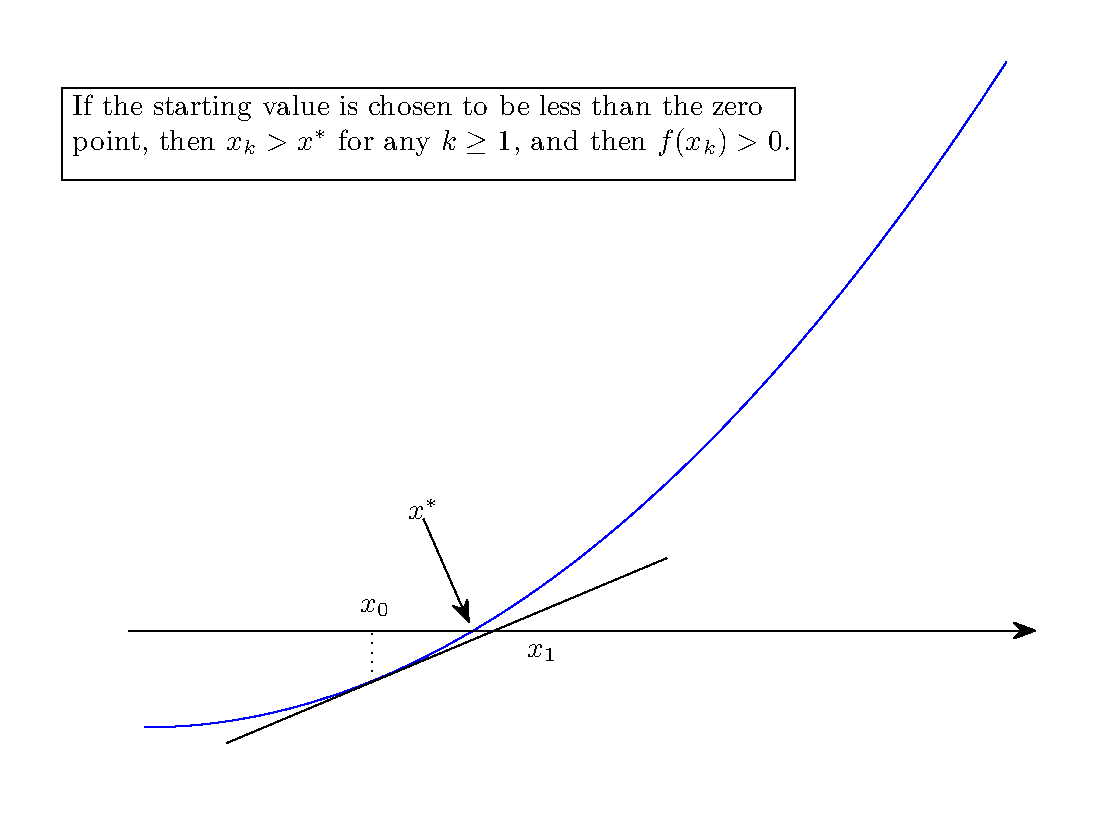
\includegraphics[width=0.7\textwidth]{\problems/\chpt/PICTURES/P2a.pdf}
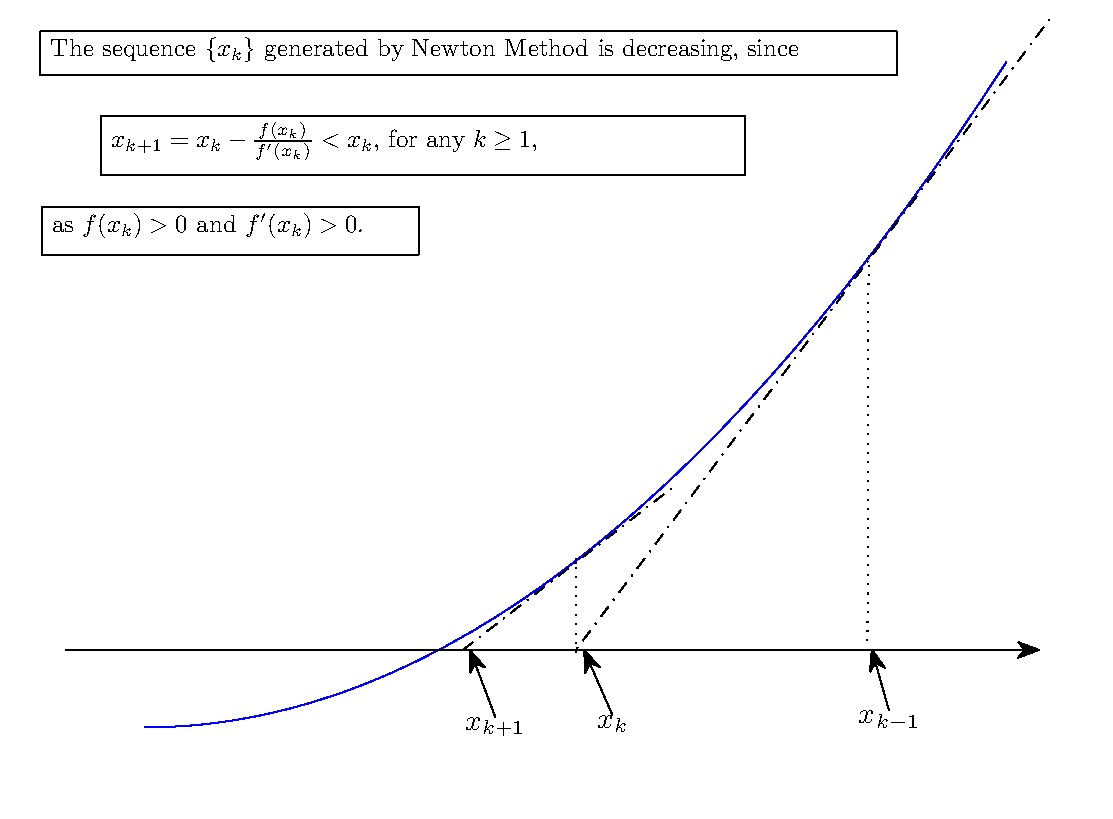
\includegraphics[width=0.7\textwidth]{\problems/\chpt/PICTURES/p2b.pdf}
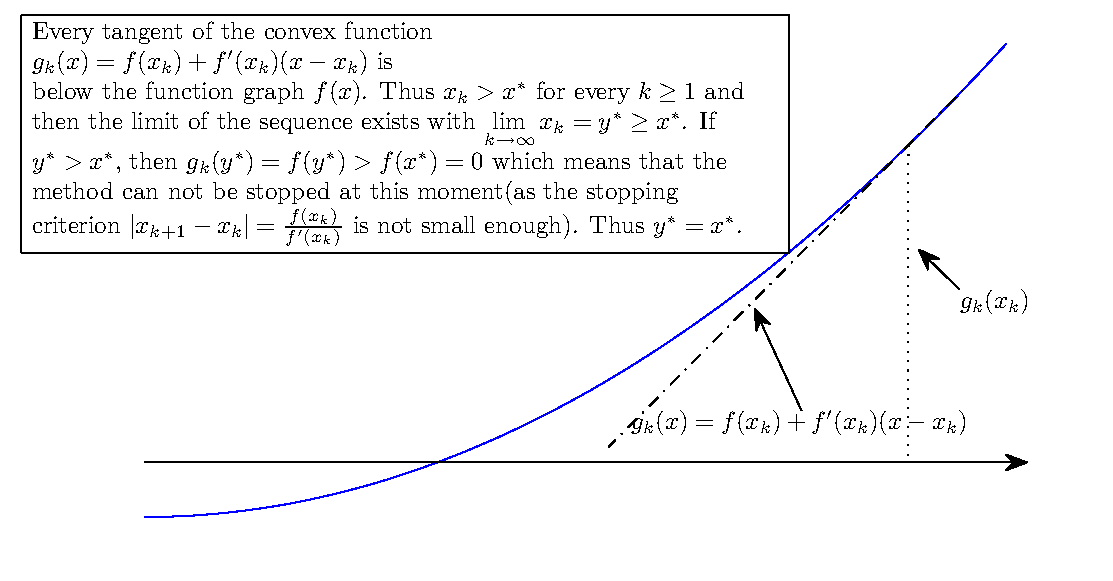
\includegraphics[width=0.7\textwidth]{\problems/\chpt/PICTURES/p2c.pdf}
\caption{Graphical proof for \ref{prb:new_iter}}
\label{fig:graph_proof_newt}
\end{centering}
\end{figure}
\end{solution}

\end{problem}